\chapter{Conclusion}
In conclusion, different MIP exact model have been developed to resolve the TSP problem and \texttt{subtour\_callback\_general} has definitely obtain the best results in term of times. However no exact algorithm can resolve a problem with more than 1000 nodes in less than 600s. This must be considered in particular when the execution time is limited. In this case heuristics can be successfully applied to obtain a good solution (not the best) about 10 times faster. This result are confirmed with the performance profile in fig \ref{fig:pp_Lbest}.\\
For the heuristics, \texttt{best\_two\_opt} obtain really good results in term of execution time and cost optimization, indeed the best heuristic are the constructive ones combined with the iteration of \texttt{best\_two\_opt}.
The constructive \texttt{n\_greedy} achieves the best performances as a heuristic alone but the use of the \texttt{n\_grasp} as a warm start brings a more variability.
\begin{figure}[!h]
	\centering
	\begin{subfigure}{.49\textwidth}
		\centering
		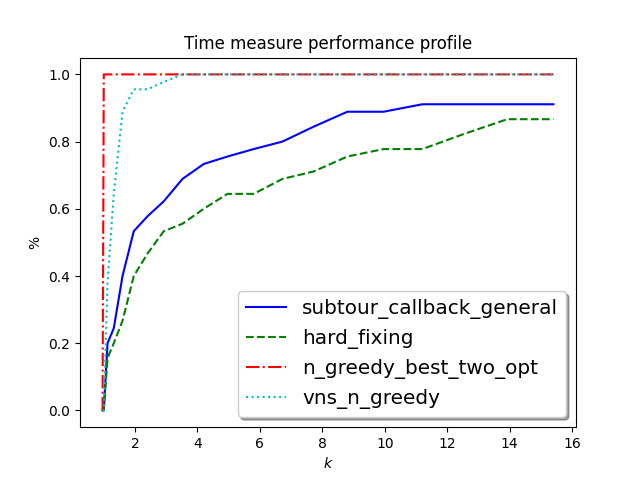
\includegraphics[width=\columnwidth]{../res/Lbest_time.png}
		\caption{Performance profile in time domain.}
		\label{fig:Lbest_time}
	\end{subfigure}
\hfill
	\begin{subfigure}{.49\textwidth}
		\centering
		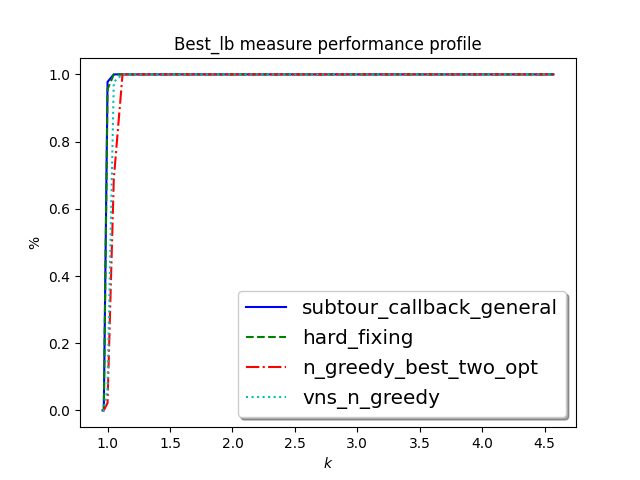
\includegraphics[width=\columnwidth]{../res/Lbest_lb.png}
		\caption{Performance profile in solution cost domain.}
		\label{fig:Lbest_lb}
	\end{subfigure}
	\caption{Performance profile of the best models executed in the union of \textit{data light} and \textit{data average}.}
	\label{fig:pp_Lbest}
\end{figure}